\documentclass[a4paper,12pt]{article}

\usepackage[slovene]{babel}
\usepackage{amsfonts,amssymb,amsmath}
\usepackage[utf8]{inputenc}
\usepackage[T1]{fontenc}
\usepackage{lmodern}
\usepackage{graphicx}
\usepackage[usenames, dvipsnames]{color}


\def\qed{$\hfill\Box$}   % konec dokaza
\def\qedm{\qquad\Box}   % konec dokaza v matematičnem načinu

\newtheorem{definicija}{Definicija}
\newtheorem{zgled}{Zgled}

\title{Grafovje in Številje}
\author{Prahmed Kavči}
\date{30.\ februar 2718}


\begin{document}

%%%%
 
\maketitle

%%%%

\section{Na Marsu}

V teoriji grafov poznamo mnogo različnih tipov grafov. Razlikujemo jih glede na njihove specifične lastnosti. V tem seminarju se bomo ukvarjali s {\em Kneserjevimi grafi} oziroma podrobneje, s {\em kromatičnim številom} le-teh. Najprej podajmo nekaj glavnih definicij.

%%%%

\begin{definicija}
{\em Graf} $G$ je urejen par $(V,E)$, kjer je $V$ množica vseh vozlišč, $E$ pa množica vseh povezav med temi vozlišči.
\end{definicija} 

\begin{definicija}
Graf $K(n,k)$, $n \geq k \geq 1$ in $n, k \in \mathbb{N}$, imenujemo \mbox{\textbf{Kneserjev}}, če je množica vozlišč $V(n,k)$ družina vseh $k$-elementnih podmnožic množice $\{1, 2, \ldots, n\}$. Dve vozlišči sta povezani natanko takrat, ko sta disjunktni. 
\end{definicija}

Povejmo še, da za število vozlišč velja $|V(n,k)|={{n}\choose{k}}$. V primeru, ko je $n < 2k$, imata vsaki dve $k$-elementni množici neprazen presek. Tak Kneserjev graf nima nobenih povezav, zato privzemimo, da velja $n \geq 2k$.


\begin{definicija}
Najmanjše število $m$, ki zadošča barvanju vozlišč grafa $G$, imenujemo \textbf {Kromatično število}. Označimo ga s $\chi(K(n,k)).$
\end{definicija}

\begin{definicija}
Preslikavo $c: V \rightarrow \{1, \ldots, m\}$, ki slika vozlišča grafa v množico barv, imenujemo \textbf {barvanje}. Ta preslikava zadošča pogoju, da sta vsaki dve sosednji vozlišči pobarvani z različnima barvama.
\end{definicija}

Kromatično število grafa $G$ je torej najmanjše število barv, s katerimi lahko pobarvamo vozlišča grafa tako, da se nobeni dve sosednji vozlišči ne slikata v isto barvo. Množico vozlišč $V$ bi radi predstavili kot disjunktno unijo barvnih razredov $V = V_1 \sqcup V_2 \sqcup \ldots \sqcup V_{\chi(G)}$, teh pa želimo, da je najmanj.
\newpage 

Oglejmo si enega najznamenitejših grafov vseh časov.

\begin{zgled}{Kneserjev graf $K(5,2)$ je zelo znan primer, imenujemo ga Petersenov graf. 

\begin{figure}[h!]
	\centering
	\begin{minipage}{0.45\textwidth}
		\centering
		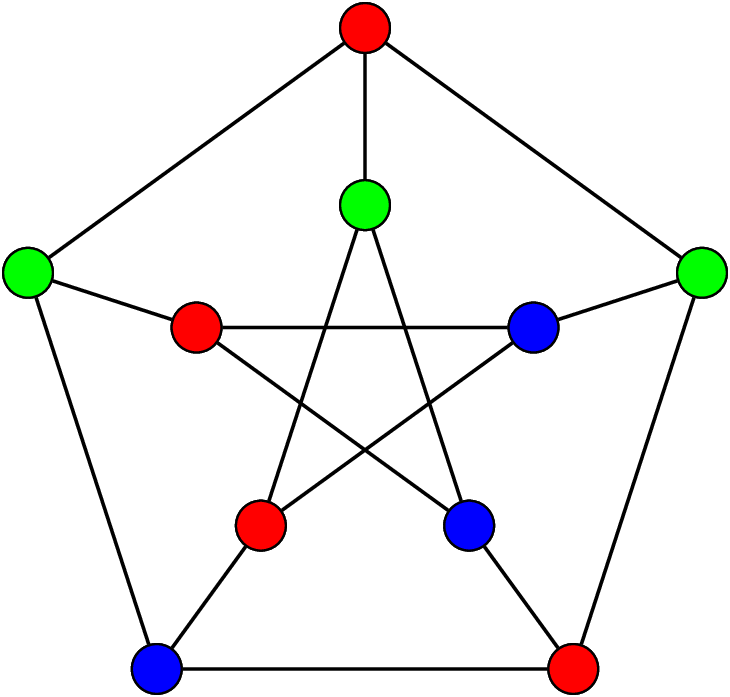
\includegraphics[width=0.8\textwidth]{petersenov_graf_barvanje}
        	\caption{Primer barvanja tega grafa z z dvema lepima barvama in \color{Green}{svetlo zeleno}}
    	\end{minipage}\hfill
    	\begin{minipage}{0.45\textwidth}
       	 \centering
        	 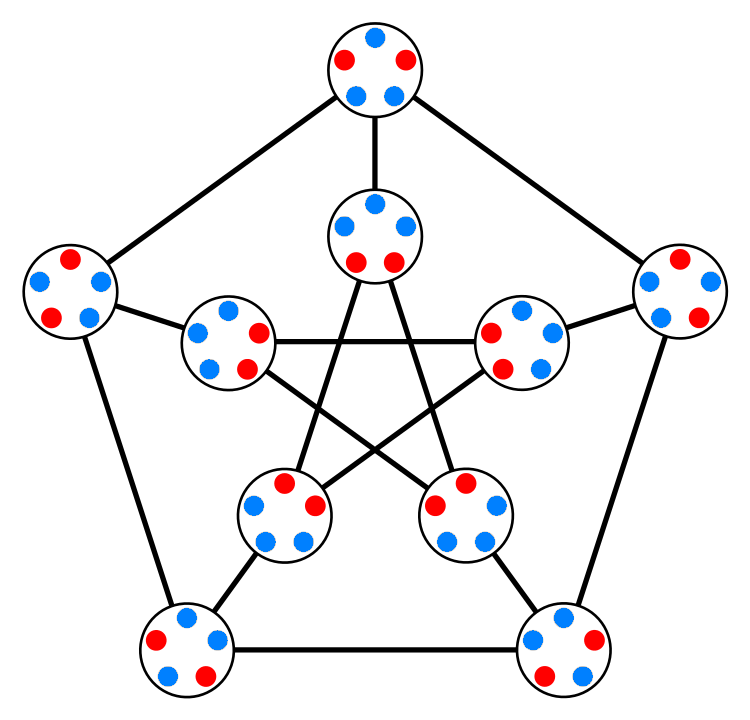
\includegraphics[width=0.8\textwidth]{petersenov_graf_mnozice}
       	 \caption{Prikaz povezav med disjunktnimi množicami}
    	\end{minipage}
\end{figure}

Ta graf zelo pogosto pride prav pri dokazovanju obstoja nekega tipa grafa ali pa kot protiprimer. Imenuje se po \textbf{Juliusu Petersenu}, ki ga je skonstruiral za najmanjši kubični graf, to je, graf, ki je regularen stopnje $3$, brez mostov in brez barvanja povezav s tremi barvami. Ima $10$ vozlišč in $15$ povezav. Če je kdo besedilo bral, ga morda zanima, kaj pomeni, da je graf regularen. Ta podatek lahko zavzet bralec najde na \\ 
\verb|https://sl.wikipedia.org/wiki/Regularni_graf|.
}
\end{zgled}

\noindent
{\color{RubineRed} \rule{\linewidth}{0.5mm} konec Marsa }

\section{Po Marsu}
Po padcu z Marsa nas je ujel Euler. Kot naš rešitelj si je privoščil predstaviti nam svojo funkcijo iz teorije števil.

\begin{definicija}
Za vse $n \in \mathbb{N}$ s $\varphi (n)$ označimo število celih števil iz množice
$\{1, 2, . . . , n\}$, ki so tuja številu $n$. Preslikavo $\varphi : \mathbb{N} \rightarrow \mathbb{N}$ imenujemo Eulerjeva
funkcija.
\end{definicija}
\newpage


\begin{table}[h!]
Tabela prikazuje izračun prvih šest vrednosti funkcije $\varphi (n)$. V $n$-ti
vrstici so krepko natisnjena števila med $1$ in $n$, ki so tuja številu $n$. Slika pa grafično prikazuje prvih $100$ vrednosti funkcije $\varphi (n)$.
\[
\begin{array}{|c||l|c|}
 n & \{1,2,\ldots, n\}          & \varphi(n)       \\
 \hline
\hline
 1 & \{{\bf 1}\}                    &     1      \\
 2 & \{{\bf 1},2 \}                &     1      \\
 3 & \{{\bf 1,2},3 \}             &     2      \\
 4 & \{{\bf 1},2,{\bf 3},4 \} &     2      \\
 5 & \{{\bf 1,2,3,4},5 \}       &     4      \\
 6 & \{{\bf 1},2,3,4,{\bf 5},6 \} &     2
\end{array}
\] 
\caption{Vrednosti funkcije $\varphi(n)$ za $n = 1,2,\ldots,6$}\label{fi}
\end{table}

\begin{figure}[h!]
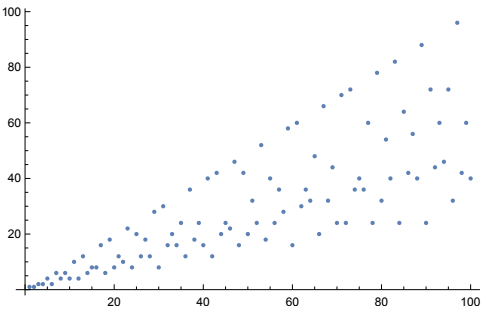
\includegraphics{eulerjeva.PNG}
\caption{Vrednosti funkcije $\varphi(n)$ za $n = 1,2,\ldots,100$}\label{fi100}
\end{figure}

\newpage
Zapišimo nekaj lastnosti te funkcije:
\begin{itemize}
\item $\varphi (mn)=\varphi (m)\varphi (n)$
\item $\varphi (n)=n \prod_{p|n}(1-\frac{1}{p})$
\item $\sum_{d|n}\varphi(d)=n$
\end{itemize}

Dokažimo, da zadnja lastnost zagotovo velja za $n=6$.

{\emph Dokaz:}
\begin{eqnarray*}
\sum_{d|6}\varphi(d) &=& \varphi(1) + \varphi(2)+\varphi(3) + \varphi(6) \\
&=& 1 + 1+2+2 \\
&=& 6
\end{eqnarray*} \qed

Brez konteksta zapišimo še eno najlepših identitet, Eulerjevo seveda:

$$e^{i\pi}+1=0.$$


\end{document}